\documentclass[12pt]{article}
\usepackage[pdftex]{graphicx}
\newcommand{\dd}{\mathrm{d}}
\newcommand{\kg}{\mathrm{kg}}
\newcommand{\m}{\mathrm{m}}
\newcommand{\cm}{\mathrm{cm}}
\newcommand{\mm}{\mathrm{mm}}
\newcommand{\km}{\mathrm{km}}
\newcommand{\mi}{\mathrm{mi}}
\newcommand{\s}{\mathrm{s}}
\newcommand{\ms}{\mathrm{ms}}
\newcommand{\h}{\mathrm{h}}
\newcommand{\N}{\mathrm{N}}
\newcommand{\W}{\mathrm{W}}
\newcommand{\hp}{\mathrm{hp}}
\newcommand{\rad}{\mathrm{rad}}
\newcounter{problem}
\stepcounter{problem}
\newcounter{answer}[problem]
\newenvironment{problem}{\noindent\begin{minipage}{\textwidth}\sloppy\sloppypar\raggedright\textbf{\theproblem.}\refstepcounter{problem}\stepcounter{answer}---}{\end{minipage}\\[2ex]}
\newcommand{\source}[1]{[{#1}]}
\newenvironment{answers}{\\[0.5ex]}{}
\newcommand{\answer}[1]{\textbf{\Alph{answer}:}\refstepcounter{answer}~\mbox{#1\hspace{3ex}}}
\newcommand{\longanswer}[1]{\textbf{\Alph{answer}:}\refstepcounter{answer}~{#1}\\}
\begin{document}

\section*{NYU General Physics 1---Term Exam 3}

\begin{problem}
  \source{from lecture 2013-10-24} You analyzed a mass $M$ sitting on
  a table-top of mass $m$ held up on two fulcra (points of contact),
  separated by a distance $L$.  If the mass $M$ is put directly over
  the \emph{left} fulcrum, what is the magnitude of the contact force
  at the \emph{right} fulcrum?  By ``contact force'' we mean the force
  of the fulcrum on the table top.
  \begin{answers}
    \answer{$\displaystyle \frac{m\,g}{2}$}
    \answer{$\displaystyle \frac{M\,g}{2}+\frac{m\,g}{2}$}
    \answer{$\displaystyle M\,g+\frac{mg}{2}$}
    \answer{$\displaystyle M\,g-\frac{mg}{2}$}
    \answer{$\displaystyle \frac{Mg}{2}$}
  \end{answers}
\end{problem}

\begin{problem}
  \source{from lecture 2013-10-29} We considered a hanging sign, with
  the cable at an angle of $\theta$ to the horizontal, as shown.
  \\\includegraphics{../mp/hanging_sign2.pdf}\\ If we choose the
  pin (black dot) connecting the beam and the wall as the axis (reference point), what is the magnitude of
  the torque on the beam coming from the cable marked ``$T_1$''?
  \begin{answers}
    \answer{$T_1\,\cos\theta$}
    \answer{$T_1\,\sin\theta$}
    \answer{$T_1\,L\,\cos\theta$}
    \answer{$T_1\,L\,\sin\theta$}
  \end{answers}
\end{problem}

\begin{problem}
  \source{from lecture 2013-10-31} Just like we did in lecture,
  consider a harmonic oscillator consisting of a mass $m$ attached to
  a spring of spring constant $k$ (force per unit length) on a
  frictionless table.  It oscillates with amplitude $A$.  The period
  of the oscillator:
  \begin{answers}
    \answer{does not depend on the amplitude}
    \answer{does not depend on the mass}
    \answer{does not depend on the spring constant}
    \answer{changes with time}
  \end{answers}
\end{problem}

\begin{problem}
  \source{from lecture 2013-11-05} We considered a stretched brass
  string of density $\rho$ and diameter $D$, fixed at both ends,
  tightened to tension $T$. Assuming $\rho$, $D$, and $T$ remain
  fixed, how does the fundamental frequency of the string depend on
  length $L$?  (Hint: As you change the length, you also change the
  total mass $M$ of the string.)
  \begin{answers}
    \answer{$f\propto 1/L$}
    \answer{$f\propto 1/\sqrt{L}$}
    \answer{$f$ is independent of $L$}
    \answer{$f\propto \sqrt{L}$}
    \answer{$f\propto L$}
  \end{answers}
\end{problem}

\begin{problem}
  \source{from lecture 2013-11-07} We discussed a traveling sinusoidal
  wave on a stretched string.  The wave moved in the $x$ direction,
  and the the bits of string oscillated in the $y$ direction.  What
  statement is \emph{false?}
  \begin{answers}
    \answer{The wave was transverse.}
    \answer{Each bit of string moves in both the $x$ and $y$ directions.}
    \answer{Every bit of string oscillates at precisely the same frequency.}
    \answer{The plots of $y$ vs time and $y$ vs $x$ were both sinusoidal in form.}
  \end{answers}
\end{problem}

\begin{problem}
  \source{from lecture 2013-11-12} The amplitude of the standing wave
  in a piano string, fixed at both ends, declines with time.  What is
  one possible reason?
  \begin{answers}
    \answer{It is subject to static friction.}
    \answer{It is under tension.}
    \answer{It is emitting a sound into the air.}
    \answer{The oscillation frequency is changing with time.}
  \end{answers}
\end{problem}

\begin{problem}
  \source{from problem set 8, problem 1} Where is the center of mass
  of this object, which you considered in the problem set?
  \\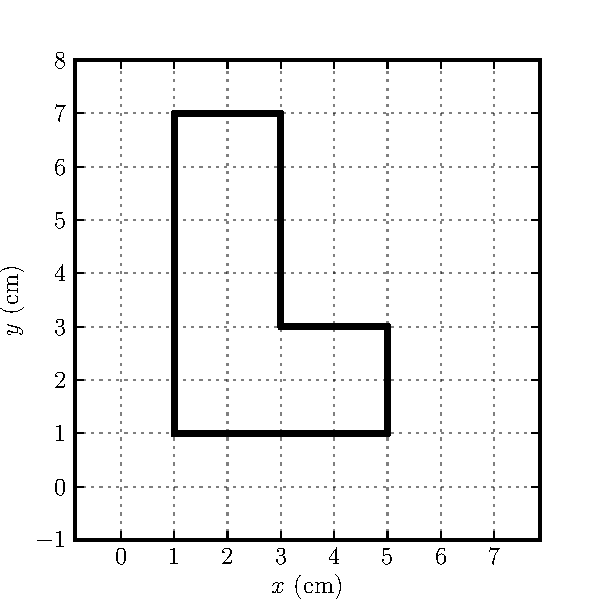
\includegraphics{../py/com_shape.pdf}
  \begin{answers}
    \answer{$x=2.5\,\cm$, $y=3.0\,\cm$}
    \answer{$x=3.0\,\cm$, $y=3.0\,\cm$}
    \answer{$x=2.5\,\cm$, $y=3.5\,\cm$}
    \answer{$x=3.0\,\cm$, $y=3.5\,\cm$}
    \answer{None of the above}
  \end{answers}
\end{problem}

\begin{problem}
  \source{from problem set 8, problem 2} Consider the topmost,
  horizontal beam in this bridge, which you considered in the problem
  set.
  \\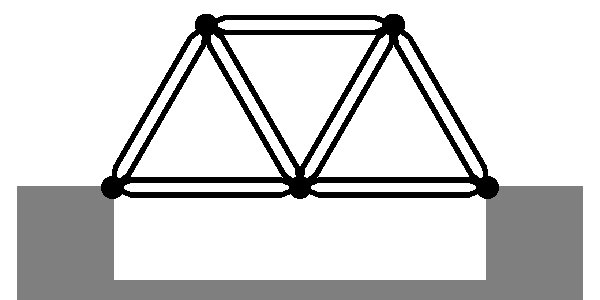
\includegraphics{../py/bridge.pdf}\\
  Is that top beam under tension or compression?  Assume that the
  joints are bearings, free to rotate!
  \begin{answers}
    \answer{tension}
    \answer{compression}
    \answer{the beam is not under stress}
    \answer{could be either, depending on other details}
  \end{answers}
\end{problem}

\begin{problem}
  \source{from problem set 8, problem 3} If you hold your right arm
  such that your upper arm is vertical and your forearm is horizontal,
  and you have a $10\,\kg$ grocery bag hanging from your right hand,
  \emph{very roughly} what is the contact force between the bones at
  your elbow joint?
  \begin{answers}
    \answer{$0.25\,\N$}
    \answer{$5\,\N$}
    \answer{$100\,\N$}
    \answer{$2000\,\N$}
  \end{answers}
\end{problem}

\begin{problem}
  \source{from problem set 9, problem 1} You solved this problem
  (ladder leaning against the wall) with two choices of ``axis of
  rotation'' or reference point.  There were some differences between
  the two calculations.  In each case you had some forces and some
  torques.  What is true about the corresponding forces and torques
  across the two calculations?
  \begin{answers}
    \longanswer{the corresponding torques and corresponding forces were all the same across the two calculations}
    \longanswer{the corresponding torques were different in the two calculations, but forces were the same}
    \longanswer{the corresponding forces were different in the two calculations, but torques were the same}
    \longanswer{the corresponding torques and forces were all different across the two calculations}
  \end{answers}
\end{problem}

\begin{problem}
  \source{from problem set 9, problem 2} A long, thin rod of length
  $L$ and cross-sectional area $A$ and elastic (Young's) modulus $E$
  has mass $M$.  Think of the rod as being like a Hooke's Law spring;
  it can be stretched by applying a force.  What is the spring
  constant $k$ for this spring?
  \begin{answers}
    \answer{$\displaystyle{E\,L}$}
    \answer{$\displaystyle\frac{E\,A}{L}$}
    \answer{$\displaystyle\frac{E}{A\,L}$}
    \answer{$\displaystyle\frac{L}{E\,A}$}
    \answer{none of these}
  \end{answers}
\end{problem}

\begin{problem}
  \source{from problem set 9, problem 2} You compared the vibration
  frequency $f_1$ of a bone supporting your mass with the pendulum
  frequency $f_2$ of the bone swinging freely under the influence of
  gravity.  What did you find?
  \begin{answers}
    \answer{$f_1 > f_2$}
    \answer{$f_1 = f_2$}
    \answer{$f_1 < f_2$}
  \end{answers}
\end{problem}

\begin{problem}
  \source{from problem set 9, problem 3} You plotted the kinetic
  energy of a simple harmonic oscillator as a function of time.  The
  plot of the kinetic energy $K$ as a function of time has what
  property?
  \begin{answers}
    \longanswer{the average kinetic energy is zero}
    \longanswer{kinetic energy increases and decreases repeatedly with time}
    \longanswer{the plot looks quadratic (like a parabola) everywhere}
    \longanswer{the kinetic energy is at a maximum when the position is at a maximum}
  \end{answers}
\end{problem}

\begin{problem}
  \source{from problem set 10, problem 1} I asked you to differentiate
  the expression
  $$ x(t) = A\,\sin(\omega\,t+\phi) $$ twice with respect to time.
  The second derivative with respect to time of this function is
  \begin{answers}
    \answer{$\displaystyle \frac{\dd^2 x}{\dd t^2} = A\,\cos(\omega\,t+\phi)$}
    \answer{$\displaystyle \frac{\dd^2 x}{\dd t^2} = -\omega^2\,A\,\sin(\omega\,t+\phi)$}
    \answer{$\displaystyle \frac{\dd^2 x}{\dd t^2} = \omega\,A\,\cos(\omega\,t+\phi)$}
    \answer{$\displaystyle \frac{\dd^2 x}{\dd t^2} = \omega^2\,A\,\sin(\omega\,t+\phi)$}
    \answer{$\displaystyle \frac{\dd^2 x}{\dd t^2} = -A\,\sin(\omega\,t+\phi)$}
  \end{answers}
\end{problem}

\begin{problem}
  \source{from problem set 10, problem 2} You made plots of the expression
  $$ y(x,t) = A\,\cos(\frac{2\pi\,x}{\lambda} - \frac{2\pi\,t}{T}) $$
  at various different times.  All these plots were sinusoidal, but
  differed from one another in what respect?
  \begin{answers}
    \answer{the amplitude was different in each plot}
    \answer{the wavelength was different in each plot}
    \answer{each plot was shifted in the $x$-direction relative to the others}
    \answer{each plot was shifted in the $y$-direction relative to the others}
  \end{answers}
\end{problem}

\begin{problem}
  \source{from problem set 10, problem 2} I gave you the expression
  $$ y(x,t) = A\,\cos(\frac{2\pi\,x}{\lambda} - \frac{2\pi\,t}{T}) $$
  where $A$, $\lambda$, and $T$ are constants. This represents a
  traveling wave. At what speed (magnitude of velocity) is it
  traveling?
  \begin{answers}
    \answer{$\displaystyle \lambda\,T$}
    \answer{$\displaystyle \frac{\lambda}{T}$}
    \answer{$\displaystyle \frac{T}{\lambda}$}
    \answer{$\displaystyle 2\,\pi\,\frac{\lambda}{T}$}
    \answer{$\displaystyle 2\,\pi\,\frac{T}{\lambda}$}
  \end{answers}
\end{problem}

\begin{problem}
  \source{from problem set 10, problem 3} The speed of sound in air is
  about
  \begin{answers}
    \answer{$0.3\,\m\,s^{-1}$}
    \answer{$3\,\m\,s^{-1}$}
    \answer{$30\,\m\,s^{-1}$}
    \answer{$300\,\m\,s^{-1}$}
  \end{answers}
\end{problem}

\begin{problem}
  \source{from \textit{Conservation of Energy} lab} You used a
  pendulum consisting of a mass on a light string.  Why does the
  tension force in the string not do any work on the mass?  That is,
  why do you not have to consider the tension force when you
  calculate the potential or kinetic energies?
  \begin{answers}
    \longanswer{The tension force is always perpendicular to the direction of motion.}
    \longanswer{The tension force is zero.}
    \longanswer{The tension force does not act on the mass.}
    \longanswer{The force of the mass on the string is opposite to the force of the string on the mass.}
  \end{answers}
\end{problem}

\begin{problem}
  \source{from \textit{Collisions in One Dimension} lab} In the lab
  you did some collision in which the lab write-up said that ``energy
  is not conserved.'' What was the more \emph{precise} meaning of this
  in the context of the lab?
  \begin{answers}
    \longanswer{The laws of physics don't hold in Meyer Hall.}
    \longanswer{Kinetic energy is not always conserved.}
    \longanswer{Momentum is not always conserved.}
    \longanswer{It is impossible to calculate the kinetic energy in these kinds of collision problems.}
  \end{answers}
\end{problem}

\begin{problem}
  \source{from \textit{Ballistic Pendulum} lab} You inferred the speed
  of the ball out of the gun by using an equation that looked like
  $$ v = D \left(\frac{g}{2\,d}\right)^{\frac{1}{2}} $$ This equation
  depends on some premises or assumptions.  Which of the following is
  \emph{not} one of those premises?
  \begin{answers}
    \longanswer{Air resistance is negligible.}
    \longanswer{The gun fires the ball horizontally.}
    \longanswer{The ball is not spinning when it is launched by the gun.}
    \longanswer{The gravitational force affects only the vertical component of velocity.}
  \end{answers}
\end{problem}

\end{document}
